\chapter{The CoastWatch Data Analysis Tool}
\label{cdatchap}
\hypertarget{cdatchap}{}

\section{Getting to know CDAT}

The CoastWatch Data Analysis Tool (CDAT) displays 2D geographic
data as a color image.  CDAT converts numerical data such as sea
surface temperature to a color map.  You can change the way data
values are converted to colors by selecting one of the various
different color palettes and by changing the data enhancement
range.  CDAT can draw coastlines, borders, latitude/longitude
grid lines, and other graphics on top of the color image.  You
can analyze the data and compute statistics by surveying at a
single point, along a line, or within a polygon.  CDAT has
features for analyzing and correcting errors in the geographic
position of the data.  Finally, CDAT can export geographic data
to a variety of image and data formats.

\begin{figure}
  \begin{center}
    \myfigure{cdat_components}
    \caption[Components of the CDAT window]{
       Components of the CDAT window
    }
    \label{cdat_components}
  \end{center}
\end{figure}

\autoref{cdat_components} shows the main components of the CDAT
window:
\begin{description}

\item[Menu bar] -- Access to file operations, tools, and the help
system.  The help system contains a short version of this
chapter, so that if you want to quickly look up a topic, you can
usually scan the help system and find it.  The tools contain a
preferences window that sets the default color palette,
enhancement range, and units for geographic data.

\item[Tool bar] -- Data file operations and view navigation.  You
can use the data file buttons to open and close files, and export
data.  More than one data file can be open at once, similar to
tabs in a web browser.  The view buttons allow you to zoom in and
out and move the view center.

\item[File tabs] -- Displays the currently open data file names,
and allows you to select the desired file.  To close a file,
select its tab and click the \button{delete}{Close} button.  You
can flip back and forth between tabs to compare data from
different files.

\item[Control tabs] -- Access to the data view control panels.

\item[Data view controls] -- The control panels are used to change
various aspects of the data view: enhancement range, color
palette, and graphics overlays.  You can also use the controls to
perform data surveys, turn on color composite mode, and correct
the geographic position (navigation correction).

\item[Variable selector] -- Displays the currently selected variable from
the data file.  You can show a new variable by selecting its name from
the drop-down list button.

\item[Data view] -- The main area showing the current geographic
data file.  The data view can show one of several variables from
a data file, for example sea surface temperature, albedo, thermal
channel data, etc.  

\item[Track bar] -- Tracks mouse movement and shows the pointer
location in latitude/longitude and image row/column coordinates,
as well as the data variable value.

\item[Color scale] -- Shows the relationship between color and data
value.  The variable name and units are also shown.  The data
values in the track bar are given in the units indicated by the
color scale.

\end{description}

\section{Loading data files}
\label{loading}

Click the \button{folder_out}{Open} button to open a data file,
and a new {\gui Open} window will appear for selecting the file
and variables to load (see \autoref{file_open}).
%%There are two
%%tabs for loading data into CDAT: \button{harddisk}{Local} and
%%\button{harddisk_network}{Network}.  Local data files are files
%%that have been downloaded and reside on the local computer, where
%%as network data files reside on an OPeNDAP data server set up for
%%serving CoastWatch data.  Most users will use the
%%\button{harddisk}{Local} tab in the {\gui Open} window after
%%downloading data from a CoastWatch web site or FTP site.
Note
that CDAT was originally designed to read CoastWatch HDF,
CoastWatch IMGMAP (no longer supported), and NOAA 1b AVHRR data files, but also reads
other formats as described in \autoref{compatible}.
%%Whether
%%using local or network data files, s
Selecting the file name
triggers the file information and variable list to change.

\begin{figure}
  \begin{center}
    \myfigure{file_open}
    \caption[File Open window]{
       File {\gui Open} window.  Windows, Unix, and Mac will show
       slightly different local file choosers (left hand panel).
       This example shows the Unix file chooser.
    }
    \label{file_open}
  \end{center}
\end{figure}

Generally data files contain more than one {\em variable}, for example
sea surface temperature (SST) data files from the AVHRR sensor contain
SST, cloud mask, visible and thermal channel data, and satellite
viewing angles.  Each {\em variable} holds a complete 2D geographic
image, and CDAT can load any combination of variables from a data
file.  Once a data file is selected, you can preview the various
variables be selecting the variable name in the list.  To load a set
of variables into CDAT, use a combination of Shift-click and
Ctrl-click (or \macsym{command}-click on Mac) and click OK.  There
will be a short delay as CDAT loads and analyzes the data in
preparation for display.  Once loaded you can change the variable
displayed using the variable selector above the data view.

When a data file is first opened, all variables are displayed
according to a set of default user preferences for the color palette,
data enhancement range, and units based on the variable name.  For
example CDAT installs with preferences that indicate the variable {\em
sst} should have the {\em HSL256} palette and an enhancement range of
-60 to 45 Celsius.  If a variable name is unknown, CDAT falls back on
a grayscale palette and a range that matches the minimum and maximum
data values found in the data.  To change these preferences for any
variable or to add new variable names to CDAT, see
\autoref{preferences} on user preferences.

% file information ?

\section{Navigating in CDAT}

CDAT displays 2D geographic data in the same way as a map, with
north in the {\em up} direction.  You can use the tool bar
buttons in combination with the mouse to zoom in and out on the
data view and move around within the view.  Following is a list
of all the actions you can perform while navigating in CDAT:
\begin{description}

\item[Zoom in] -- There are three ways to zoom in: (i) click
the \button{selection_view}{Zoom} button to enter zoom mode and
drag on the view to draw a rectangle to magnify, (ii) click the
\button{zoom_in}{Magnify} button to magnify the view $\times$2,
or (iii) click the \button{view_1_1}{Actual} button to make data
pixels the same size as screen pixels.

\item[Zoom out] -- To zoom out, click the
\button{zoom_out}{Shrink} button to shrink the view $\times$2.

\item[Move around] -- There are two ways to move around
within the view: (i) click the \button{signpost}{Pan} button to
enter pan mode and drag on the view to move it, or (ii) click the
\button{flash}{Recenter} button to enter recentering mode and
click the view to recenter on the mouse cursor.

\item[Reset] -- There are two ways to reset the view,
depending on the desired effect: (i) click the
\button{undo}{Reset} button to completely reset the view so that
all data is displayed, or (ii) click the
\button{fit_to_size}{Fit} button to fit as much data as possible
into the view area so that the view is completely filled (some
edges of the data may be cropped off).

\end{description}

\section{Changing data image colors}
\label{changing_colors}

The CoastWatch Data Analysis Tool creates a color image from 2D
geographic data by converting data values to colors using a color
palette, enhancement range, and enhancement function.  The
control tabs hold two sets of controls that are used to change
the way data values are converted to colors: the
\button{column-chart}{Color Enhancement} tab and the
\button{palette}{Color Palette} tab (see \autoref{color_tabs}).
\autoref{enhancement} shows the two step process: (i)
normalization of data values using an enhancement function, and
(ii) conversion of normalized values to colors.  Typically a
linear enhancement function is used so that the minimum and
maximum range values map to 0 and 1 respectively, and all data
values in the range are scaled linearly between 0 and 1.  In
contrast, a log function scales data values by powers of ten, for
example if the range is $[0.01..100]$, 0.1 scales to 0.25, 1
scales to 0.5, and 10 scales to 0.75.

\begin{figure}
  \begin{center}
    \myfigure{color_tabs}
    \caption[Color conversion tabs]{
       Color conversion tabs.  (a) Controls for the enhancement
       function and range.  (b) Controls for palette
       selection.
    }
    \label{color_tabs}
  \end{center}
\end{figure}

\begin{figure}
  \begin{center}
    \myfigure{enhancement}
    \caption[Color enhancement process]{
       Color enhancement process.  Two steps are performed, first
       the enhancement function is applied, and then the color
       palette.
    }
    \label{enhancement}
  \end{center}
\end{figure}

The \button{column-chart}{Color Enhancement} tab has a number of
controls to change the enhancement range and function.  Use the
sliders to change the range visually, or enter numbers into the
minimum/maximum text fields and press Enter.  The data histogram
is a visual guide that shows where most of the data values lie --
move the sliders to above and below the major histogram peaks to
see the data with the best possible color contrast.  To simplify
setting the range, the {\gui Normalize} button changes the range
to bracket the data mean with a 1.5 standard deviation unit
window, the {\gui Reverse} button swaps the minimum and maximum
range values, and the {\gui Reset} button sets the range back to
its full extents.  The enhancement function can be: (i) {\gui Linear},
(ii) {\gui Log10} for log base 10 as described above, (iii) {\gui Step} 
for a linear function with discrete steps, or (iv) {\gui Gamma} for brightness
data (0\% - 100\%) that needs a correction for computer displays.

The \button{palette}{Color Palette} tab shows the current color
palette and list of available palettes.  CDAT comes installed
with a number of palettes but users can also add their own
palettes in an XML text format as described in
\autoref{preferences}.

\section{Displaying coastlines, grids, and more}

The CoastWatch Data Analysis Tool uses graphics {\em overlays} to
show reference lines like latitude and longitude, coastlines,
political borders, bathymetry, and topography, as well as mask
data such as cloud masks.  Overlays are arranged in {\em layers}
like overhead projector slides -- most of each layer is
transparent except where the graphics occur and graphics from an
upper layer are drawn on top of graphics from a lower layer as
shown in \autoref{layers}.  Overlays can be added and removed,
turned on and off, their layering order rearranged, and their
properties modified such as color, font style, and line style.
The \button{tables}{Overlay Layers} tab holds the overlay
controls as shown in \autoref{overlays_tab}.

\begin{figure}
  \begin{center}
    \myfigure{layers}
    \caption[Overlay graphics drawing order]{
       Overlay graphics drawing order.
    }
    \label{layers}
  \end{center}
\end{figure}

\begin{figure}
  \begin{center}
    \myfigure{overlays_tab}
    \caption[Overlay Layers tab]{
       \button{tables}{Overlay Layers} tab
    }
    \label{overlays_tab}
  \end{center}
\end{figure}

\subsection{Types of overlays}

Several different types of overlays can be added to the data
view.  In general, any overlay can have a custom color and
transparency, and line overlays can have custom line style, font,
and drop shadow settings.
\begin{description}

\item[\button{table}{Grid}] -- Grid lines of two different types:
\begin{itemize}

  \item \button{environment}{Lat/Lon} -- Latitude and longitude
  lines.  The default is to render labeled lines at regular
  increments based on the zoom factor, but you can customize the
  line increment value and labels.

  \item \button{cube_molecule}{Data reference} -- Row and column
  lines that follow the image data.  The default is to render
  labeled lines at regular increments based on the zoom factor,
  but you can set the line placement and customize the labeling.

\end{itemize}

\item[\button{earth2}{Coast}] -- Land/water boundaries including
oceans, lakes, islands in lakes, and ponds in islands derived
from the Global Self-consistent Hierarchical High-resolution
Shorelines (GSHHS) data set:
\url{http://www.ngdc.noaa.gov/mgg/shorelines/gshhs.html}.  The
resolution of the lines drawn depends on the zoom factor of the
data view and ranges from 25 km (crude resolution) to 0.2 km
(high resolution).  Land polygons can be drawn by specifying a
fill color.

\item[\button{flag_red}{Political}] -- International and state
border lines derived from CIA WDB-II data.  As with coastline
data, the resolution of the lines changes with the data view
zoom.  Only international borders are shown by default -- you can
add state borders manually.

\item[\button{photo_scenery}{Topography}] -- Topographic and
bathymetric lines contoured in real-time from ETOPO5 elevation
data: \url{https://www.ngdc.noaa.gov/mgg/global/etopo5.HTML}.
Only the 200~m and 2000~m bathymetric contours are shown by
default.  The topography levels can be modified to include any
set of topographic or bathymetric contours.

\item[\button{masks}{Mask}] -- One of three different types
of masks:
\begin{itemize}

  \item \button{cubes_green}{Bitmask} -- A single-color mask that
  uses a bitwise AND operation.  A bitmask uses data values from
  a variable and performs a bitwise AND with each data value and
  an integer mask value to determine which pixels in the data
  view should be masked.  If the results of the AND operation are
  non-zero, the pixel if masked otherwise is is left unmasked.
  Suppose that an integer data variable named ``cloud'' contains
  a value of 0 when no clouds are present, or a value of 1 when
  clouds are detected at a pixel.  Then a bitmask with an integer
  mask value of 1 will cover all cloud pixels with the mask
  color.  More complex masking can also be achieved -- for
  example, suppose a variable named ``graphics'' has the fourth
  bit set when land is present at the pixel.  Then a bitmask with
  an integer mask value of 8 will select out all graphics pixels
  with the fourth bit set in order to mask only land pixels.

  \item \button{cubes}{Multilayer} -- A multiple-color mask that
  combines a set of single-color bitmasks.  A multilayer mask
  uses data values from a variable and colors each bit set to 1
  in the data value with a different color.  The idea is that if
  none or only a few of the bits in each data value are set, the
  mask will let the data show through in most locations and mask
  it with a bit-identifying color in others.  This is useful when
  working with data analysis output such as cloud masking where
  each bit in an integer data value represents the output from a
  different cloud mask test.  A multilayer mask can handle up to
  32 different colors, one color for each bit in a 32-bit integer
  data value.

  \item \button{calculator}{Expression mask} -- A single-color
  mask that uses a boolean expression.  An expression mask
  evaluates a boolean expression and masks any pixels for which
  the expression is true.  Expression masks are slower to compute
  than bitmasks or multilayer masks, but are much more flexible
  because almost any mathematical combination of data variable
  values can be used.  For example, an expression mask with the
  mask expression of ``sst $<$ 5'' will mask out all SST
  temperature data values less than 5 degrees.  Any mathematical
  operator or constant supported by the
  \hyperlink{cwmath}{cwmath} tool can be used in the expression,
  as long as the variables referenced in the expression were
  imported when the data file was loaded.

\end{itemize}

\item[\button{shapes}{Shape}] -- Shape data lines stored in ESRI
shapefile format. Shape overlays are limited in a number of ways:
(i) only line and polygon shape data is rendered (no point data),
(ii) shape overlays cannot be saved as part of an overlay group,
and (iii) rendering may be slow for large and complex shapefiles.

\end{description}

\subsection{The {\gui Overlay List}}
\label{overlay_list}

Overlays are added by clicking one of the buttons from the
{\gui Add Overlay} area of the \button{tables}{Overlay Layers}
tab.  When an overlay is first added to the data view, it's given
a default set of properties (line style, line color, fill color,
etc.) and appears in the {\gui Overlay List} area.  You can change
any of the basic overlay properties by just clicking the property
in the list, or change some of the more complex and
overlay-specific properties by selecting the overlay and clicking
the \button{document_edit}{Edit Properties} button
(double-clicking the overlay also brings up the full property
editor).

Since overlays are layered like overhead projector slides, their
order can be changed using the \button{arrow_up_green}{Move Up}
and \button{arrow_down_green}{Move Down} buttons.  They can be
set temporarily invisible with the {\gui Visibility} check box, or
deleted altogether using \button{delete}{Delete}.

\subsection{Overlay groups}

The {\gui Overlay Groups} area of the tab lets you save and
restore a set of overlays that you frequently use.  Overlay
groups are useful for when you've created a complex set of
overlays, arranged them into the correct order, changed their
properties, and want to use them again for another data file.  A
default set of overlay groups are provided when CDAT is installed
(see \autoref{overlay_groups}):
\begin{description}

\item[{\gui Atmospheric}] -- Latitude/longitude grid lines, coast,
and state/international borders for use on atmospheric data with
a grayscale palette.

\item[{\gui Oceanographic}] -- Latitude/longitude grid lines,
coast with filled land polygons, state and international borders
for use on oceanographic data with a color palette.

\item[{\gui Oceanographic - Cloud Analysis}] -- The same overlays
as Oceanographic, with extra cloud analysis overlays for NOAA
NESDIS SST product users.

\item[{\gui Oceanographic - Coral Reef Watch}] -- Special overlays
customized for use with Coral Reef Watch data (see the Coral Reef
Watch page at \url{http://coralreefwatch.noaa.gov} for data and
other details).

\end{description}

\begin{figure}
  \begin{center}
    \myfigure{overlay_groups}
    \caption[Examples of default overlay groups]{
       Examples of default overlay groups.  The grayscale image
       shows the {\gui Atmospheric} overlay group, while the color image
       shows {\gui Oceanographic - Cloud Analysis}.
    }
    \label{overlay_groups}
  \end{center}
\end{figure}

To use one of the default groups, select it in the list and click
the \button{folder_out}{Open Group} button.  The overlays are
loaded into the overlay list on top of any existing overlays.  To
create a new overlay group, select a set of overlays from the
{\gui Overlay List} using Shift-click and Ctrl-click
(\macsym{command}-click on Mac), then click the
\button{disk_blue}{Save Group} button.  You can create a new
overlay group by typing in a new name, or replace an existing
overlay group.  To remove an unwanted overlay group, select it
and click \button{delete}{Delete Group}.

Another useful feature of overlay groups is that once created,
they can be used for command line data rendering by specifying
the \longoption{group} option in the
\hyperlink{cwrender}{cwrender} tool.  Overlay groups are saved in
a special directory on a per-user basis along with other user
preferences as described in \autoref{preferences}.

\section{Measuring distances and data statistics}
\label{surveys}

CDAT can be used perform several different types of surveys of
the current variable in the data view.  The
\button{tape_measure2}{Data Surveys} tab (\autoref{surveys_tab})
allows you to manage a list of surveys and create new ones by
selecting areas of the data view.  Each data survey performed
results in a set of data statistics, survey dimensions such as
endpoints and distances, and a line or histogram plot.

\begin{figure}
  \begin{center}
    \myfigure{surveys_tab}
    \caption[Data Surveys tab]{
       \button{tape_measure2}{Data Surveys} tab
    }
    \label{surveys_tab}
  \end{center}
\end{figure}

\subsection{Types of surveys}

To perform a survey, select one of the {\gui Survey Mode} buttons
and click on the data view as follows:
\begin{description}

\item[\button{pin_blue}{Point}] (single click) \\ A single point
survey with only the point position and data value reported but
no statistics or plot.  A point survey is a good way to mark a
certain position and easily be able to recall its data value,
such as for an ocean buoy.  Point surveys are marked with a small
cross.

\item[\button{bullet_ball_glass_blue_line}{Line}] (click/drag) \\
A straight line survey with the line endpoint positions, distance
in kilometers, statistics, and an X-Y plot of the data values
along the line. A line survey simulates an airplane or ship track
of the data values, and is useful for gradient and front
analysis.

\item[\button{bullet_ball_glass_blue_box}{Box}] (click/drag) \\ A
rectangular box survey, with the box corner point positions,
statistics, and a histogram plot of the data within the box. A
box survey is useful for a clustering analysis to show groups of
similar data values in an area as peaks in the histogram.

\item[\button{bullet_ball_glass_blue_polygon}{Polygon}] (click
corners / double-click last corner) \\ A polygon survey with
statistics and a histogram plot of the data within the
polygon. Polygon surveys are similar to box surveys, but can help
when the area has an irregular shape.

\end{description}

\subsection{The {\gui Survey List} and results}

When you perform a data survey, a new entry is added to the
{\gui Survey List} area that shows the survey name and line
properties.  By default surveys are marked by thick red lines but
the line color and style can easily be changed to more easily see
the difference between similar surveys.  Surveys can be
temporarily hidden and shown again by clicking the
{\gui Visibility} check box, or deleted using
\button{delete}{Delete}.  The {\gui Survey List} area is very
similar in usage to the {\gui Overlay List} area in the
\button{tables}{Overlay Layers} tab (see \autoref{overlay_list}).

Selecting an entry in the survey list changes the {\gui Results}
and {\gui Plot} tabs to display the results of the survey.  For
line surveys all data values along the line are sampled and the
statistics reported.  For box and polygon surveys, CDAT attempts
to speed up statistics computations by only sampling 1\% of the
data values although this may not always be possible for smaller
areas.  The statistics reported are as follows:
\begin{description}

\item[{\gui Sample}] -- For box and polygon surveys only, the
number of data values sampled as a percentage of the total number
of data values in the survey area.

\item[{\gui Count}] -- The total number of data values sampled.

\item[{\gui Valid}] -- The total number of data values encountered
that were not marked as missing.  Missing data values are skipped
by the statistics computations.  In many cases data values are
marked as missing prior to being written to the data file for
data quality reasons.

\item[{\gui Min}] -- The minimum valid data value sampled.

\item[{\gui Max}] -- The maximum valid data value sampled.

\item[{\gui Mean}] -- The mean of all valid data values sampled.

\item[{\gui Stdev}] -- The standard deviation from the mean of all
valid data values sampled.

\end{description}
Line survey plots show the data value as a function of the pixel
distance along the line.  Box and polygon survey plots show a
normalized histogram bin count as a function of the data value.

\section{Drawing lines, shapes, and text}

The CoastWatch Data Analysis Tool can be used to draw lines,
boxes, circles, curves, and text on the data view.  When the data
view is exported to an image file, the annotations are drawn as
well; annotations are an easy way to create example images for
presentations that highlight features of interest in the data.
The \button{pda_write}{Annotations} tab
(\autoref{annotations_tab}) allows you to pick the annotation
mode and manage a list of annotations on the data view.

\begin{figure}
  \begin{center}
    \myfigure{annotations_tab}
    \caption[Annotations tab]{
       \button{pda_write}{Annotations} tab
    }
    \label{annotations_tab}
  \end{center}
\end{figure}

\subsection{Types of annotations}

To add an annotation to the data view, click one of the
{\gui Annotation Tool} buttons and add it to the data view as
follows:
\begin{description}

\item[\button{bullet_ball_glass_blue_line}{Line}] (click/drag) \\
Draws a line in the current color and style.

\item[\button{bullet_ball_glass_blue_polyline}{Polyline}] (click
endpoints / double-click last point) \\ Draws a series of
connected line segments in the current color and style.

\item[\button{bullet_ball_glass_blue_box}{Box}] (click/drag) \\
Draws a rectangular box in the current color and style, and fills
with the fill color.

\item[\button{bullet_ball_glass_blue_polygon}{Polygon}] (click
corners / double-click last corner) \\ Draws an irregular polygon
in the current color and style, and fills with the fill color.

\item[\button{bullet_ball_glass_blue_circle}{Circle}]
(click/drag) \\ Draws a circle from the center to radius point in
the current color and style, and fills with the fill color.

\item[\button{bullet_ball_glass_blue_curve}{Curve}] (click
control points / double-click last point) \\ Uses a set of
polyline control points to draw a Bezier curve in the current
color and style.

\item[\button{font}{Text}] (click and enter text) \\ Places the
specified text in the current font and color. The text font size
is relative to the screen, and so remains constant if the data
view zoom factor is modified. The text anchor point moves with
the view.

\end{description}

\subsection{The {\gui Annotation List}}

When creating an annotation, a new entry is added to the
{\gui Annotation List} according to the current {\gui Drawing
Defaults} settings.  Similar to overlays and surveys, annotation
layers can be hidden/shown, deleted, rearranged, and edited (see
\autoref{overlay_list}).

\section{Using composite image mode}

CDAT normally displays 2D geographic data as a color image by
mapping the data values of a variable to colors using a color
palette.  Rather than using a palette, an alternative way of
deriving the color values at each pixel is to treat data values
from different variables as components of a color.  CDAT uses the
RGB color model (see \url{http://en.wikipedia.org/wiki/RGB}) to
combine data from three different variables to form the pixel
colors.  The process of converting data values to color
components is similar to that shown in \autoref{enhancement} but
rather than converting the normalized value to a palette color in
the second step, the normalized value is used as the intensity of
red, green, or blue in the pixel color.  

\begin{figure}
  \begin{center}
    \myfigure{composite_tab}
    \caption[Color Composite tab]{
       \button{colors}{Color Composite} tab
    }
    \label{composite_tab}
  \end{center}
\end{figure}

The \button{colors}{Color Composite} tab
(\autoref{composite_tab}) contains controls for choosing the
variables to use as components, and for turning on/off color
composite mode.  To create a color composite:
\begin{enumerate}

\item Choose three variables from those imported when the data
file was opened.  Set the variables as the {\gui Red},
{\gui Green}, and {\gui Blue} components in the
\button{colors}{Color Composite} tab.  The best choice of
variables depends on the data -- satellite data channels of
different wavelengths work well as long as the three channels are
reasonably independent.

\item Use the variable selector (see \autoref{cdat_components})
to view each variable and set up the enhancement function in the
\button{column-chart}{Color Enhancement} tab.  The easiest way to
set up the enhancement function is to use a grayscale palette to
visually judge the scene contrast and click {\gui Normalize} which
centers the enhancement function around the mean.  Then use the
range sliders to fine tune the enhancement.

\item Click the {\gui Perform color composite} check box in the
\button{colors}{Color Composite} tab to turn composite mode on.
While in composite mode you can continue to select variables and
change their enhancement functions to obtain the best mixture of
color components.

\end{enumerate}

\autoref{rgb_example} shows examples of RGB color composite
images created using NOAA AVHRR data and Chinese FY-1D MVISR
data.

\begin{figure}
  \begin{center}
    \myfigure{rgb_example}
    \caption[RGB composite examples]{
       RGB composite examples.  (a) NOAA-18 AVHRR false color
       composite using channels 1/2/4.  (b) FY-1D MVISR true
       color composite using channels 1/9/7.
    }
    \label{rgb_example}
  \end{center}
\end{figure}

\section{Correcting geographic location problems}

The CoastWatch Data Analysis Tool was written in part for
NOAA/NESDIS researchers to use in evaluating the quality of
satellite data products.  One of the quality measures is computed
satellite angle data ({\em navigation} data) including latitude,
longitude, solar zenith, satellite zenith, and relative azimuth
angles.  Of particular interest are latitude and longitude because
uncertainty in those angles determines the positional accuracy of
the data.  For example if the latitude and longitude of a pixel
have an uncertainty of 0.01$^{\circ}$ then the pixel has a
positional accuracy of $\sim$1~km.  Small uncertainties such as
these can exist when a satellite's true orientation and position
are not known exactly. In this case the image data in CDAT may
not line up correctly with coastline overlays. The image may
appear to be shifted, rotated, or sheared in comparison to the
coastlines.  Navigation errors are not as prevalent if the data
file has been produced recently, but are not uncommon in older
data files or in experimental satellite data products.

There are two tools in CDAT designed for working with navigation
data errors: the \button{environment_ok}{Navigation Correction}
tab and the {\gui Navigation Analysis} panel.  Navigation
correction writes a set of correction parameters to a data file
so that subsequent data access using the CoastWatch Utilities
takes into account the correction.  Navigation analysis allows
you to examine the navigation accuracy of various points in the
data file and save point position, variable data, and navigation
offsets for later analysis.

\subsection{Navigation correction}

The \button{environment_ok}{Navigation Correction} tab (see
\autoref{navigation_tab}) is used to write correction parameters
to a data file so that the data view image lines up correctly
with actual geographic features such as coastlines.  Only data
files in CoastWatch HDF (.hdf)
format can be corrected.  Also, only satellite sensor and
sensor-derived variables in a data file should be corrected --
not latitude/longitude data, graphics, or viewing angle data. You
must select which specific variables to correct using the
{\gui Correction Variables} list (default is all variables
imported when the file was opened).  Navigation corrections will
only be applied to the selected variables in the list.  Examples
of data variables that may require correction include AVHRR
channel data, SST and cloud. \autoref{correction} shows an
example of an uncorrected and corrected albedo image.

\begin{figure}
  \begin{center}
    \myfigure{navigation_tab}
    \caption[Navigation Correction tab]{
       \button{environment_ok}{Navigation Correction} tab
    }
    \label{navigation_tab}
  \end{center}
\end{figure}

\begin{figure}
  \begin{center}
    \myfigure{correction}
    \caption[Navigation correction example]{
       Navigation correction example.  (a) Visible channel albedo
       image before navigation correction.  (b) Image after
       translation correction.
    }
    \label{correction}
  \end{center}
\end{figure}

You can perform a navigation correction in one of two ways:
\begin{description}

\item[Visually] -- Click one of the {\gui Visual Correction} buttons,
either \button{elements1}{Translation} or
\button{element_replace}{Rotation}.
\button{elements1}{Translation} mode corrects the navigation by
shifting the entire image in the row and column directions --
click and drag anywhere on the data view to shift the origin.
\button{element_replace}{Rotation} mode corrects the navigation
by rotating around the center of the data view -- click on an
edge of the view and drag to rotate.

\item[Manually] -- Select the type of transformation, fill in the
parameters, and click {\gui Perform} to correct the navigation.
The {\gui translation transform} is similar to the visual
translation mode -- it shifts the data origin by some number of
rows and columns.  The {\gui rotation transform} is more general
than the visual rotation mode because the rotation center point
row and column can be specified rather than having to use the
data view center.  The {\gui general affine transform} is the most
general of all (it has no visual mode counterpart) because it can
be used to correct for translation, rotation, skew, and scaling
problems.  The affine transform is applied to the row and column
coordinates of each data view pixel to translate the ``desired''
row and column coordinates $(R',C')$ to the ``actual''
coordinates $(R,C)$ in the data file:
\[
  \left[ \begin{array}{c}
           R' \\
           C' \\
           1
         \end{array}  
  \right]
  = 
  \left[ \begin{array}{ccc}
           a & c & e \\
           b & d & f \\
           0 & 0 & 1
         \end{array}
  \right]
  \left[ \begin{array}{c}
           R \\
           C \\
           1
         \end{array}
  \right] .
\]
\end{description}
To completely remove the navigation correction on a variable,
click {\gui Reset correction to identity} and then {\gui Perform}.
More information about how navigation corrections
are stored in CoastWatch HDF data files can be found in
\autoref{metadata}.  Command line tools for performing navigation
correction from a script rather than interactively are described
in \autoref{registration}, and in more detail in the
\hyperlink{cwnavigate}{cwnavigate} and
\hyperlink{cwautonav}{cwautonav} manual pages.

\subsection{Navigation analysis}
\label{nav_analysis_section}

The {\gui Navigation Analysis} panel shown in
\autoref{navigation_analysis} is accessed from the {\gui Tools}
menu and enables researchers to gather statistics on navigation
errors for a series of points in a data file.  You can compare
the known coastline geography from GSHHS coastline data to the
data view image coastline to check for navigation errors.  The
panel shows a list of navigation points and allows you to add new
points to the list, adjust the navigation offset for each point,
and save the points to a data file.

\begin{figure}
  \begin{center}
    \myfigure{navigation_analysis}
    \caption[Navigation Analysis panel]{
       {\gui Navigation Analysis} panel
    }
    \label{navigation_analysis}
  \end{center}
\end{figure}

There are two modes for adding new navigation points to the list,
both of which work by clicking on the data view in the main CDAT
window to select the point location.  \button{pin_green}{Manual}
mode adds a point to the list and lets the user adjust the
navigation offset manually.  \button{magic-wand}{Automatic} mode
adds a point to the list and additionally runs the image data in
the box surrounding the point through an automatic navigation
algorithm that attempts to: (i) classify the image data into land
and water based on histogram splitting, and (ii) compute an
optimal offset for the navigation box by finding the offset with
maximum correlation between classified image data and
pre-computed land mask data.  The automatic navigation algorithm
can sometimes fail to find a significant correlation at any
offset in which case the {\gui Status} column indicates
\textcolor{red}{{\gui Auto failed}} otherwise it indicates
\textcolor{green}{{\gui Auto OK}}.

Once a series of points are added to the list, the navigation
offset of each point can be adjusted.  Even if the automatic
navigation algorithm was successful, it may be necessary to
manually adjust the offsets -- the algorithm is only capable of
returning integer-valued offsets and some cases may require
fractional offsets for the best coastline fit.  To adjust the
offset of a point, select the point in the list and click/drag on
the offset image or use the row and column offset adjustment
controls.  You can change the variable shown in the offset image
and the navigation box size to better see the contrast between
land and water.  The {\gui Variable} and {\gui Box size} controls
also determine what data is used for automatic navigation when
adding new points.  Click {\gui Auto} to re-try the automatic
navigation algorithm after changing the variable or box size, or
{\gui Reset} to set the offset back to zero.  Navigation points
are removed from the list by clicking \button{delete}{Delete}, or
the point list cleared entirely by clicking {\gui Clear}.

After adding navigation points to the list and adjusting their
offsets if needed, the point locations (latitude, longitude, row,
column), navigation offset (row and column), variable data
values, and other metadata can be saved to a text file.  There
are two output formats: XML (structured markup language) and CSV
(comma separated value).  The XML format writes out each point
using XML tags and attributes and is useful for web browser
display and XML readers.  The CSV format writes each point as a
line of comma separated values, ready for input to a spreadsheet
or plotting program.  Examples of each format can be found in
\autoref{misc_formats}.

To save navigation points, click {\gui Save...} and choose:
\begin{itemize}
 
  \item Points to save (default is all points)

  \item Variable data values (default is no variable data)

  \item Output format (default is XML)

  \item File name and location

\end{itemize}
Regardless of the output format, the following data is saved for
each point:
\begin{description}

  \item[Earth location] -- The latitude (-90..90) and longitude
  (-180..180) of the point in degrees.

  \item[Data location] -- The row and column of the point in the
  data file, referenced from (0,0).

  \item[North direction] -- The direction of north for the point
  as a unit vector with row and column components.  This is
  useful for recovering satellite projection information at the
  point.

  \item[Navigation offset] -- The navigation offset of the point
  in the row and column directions.

  \item[Comment] -- The value of the status column indicating
  {\gui Manual}, {\gui Auto OK}, or {\gui Auto failed}.

  \item[Variable values] -- A data value for each variable
  selected in the save dialog.

\end{description}

\section{Exporting images and data}
\label{exporting}

CDAT can export either the main data view (a color image with
color scale and information legends) or the data file values and
metadata (character, integer, floating point values).  How the
exported data is to be used determines the format -- {\em color
image formats} such as PNG and JPEG are commonly used for
creating graphics for the web, printable materials, or
presentation slides for meetings while {\em numerical data
formats} such as HDF, NetCDF, and ArcGIS are used for getting data into
other analysis or GIS software packages.

To export the current data view to a color image, click the
\button{export2}{Export} button and select one of the image
formats: PNG (the default), GIF, JPEG, GeoTIFF, or PDF.  Each
format has certain characteristics:
\begin{description}

\item[PNG] -- A non-lossy compressed image format supported by
most web browsers and image manipulation software. PNG has
similar data compression characteristics to GIF and additionally
supports 24-bit color images.

\item[GIF] -- A non-lossy compressed format also supported by most
web browsers and image manipulation software. The GIF files
produced use LZW compression. Images stored in GIF format are run
through a color quantization algorithm to reduce the color map to
256 colors or less. Although file sizes are generally smaller
than PNG, image quality may be compromised by the reduced color
map.

\item[JPEG] -- A lossy compressed format that should be used with
caution for images with sharp color lines such as those found in
text and annotation graphics. The JPEG format generally achieves
higher compression than PNG or GIF resulting in smaller image
file sizes.

\item[GeoTIFF] -- A flexible image format with support for earth
location metadata. Many popular GIS packages handle GeoTIFF
images and allow the user to combine a GeoTIFF base map image
with other sources of raster and vector data. The GeoTIFF images
generated are non-lossy uncompressed image data (unless a
compression is specified in the options), and can be much larger
than the corresponding PNG, GIF, or JPEG. In general the GeoTIFFs
generated are 24-bit colour images, but when no overlays are used
or the image color option is set, a special 8-bit paletted image
file is generated and comments describing the data value scaling
equation are inserting into the image description tags. Note that
the \hyperlink{cwexport}{cwexport} command line tool also creates
GeoTIFF files that contain 32-bit IEEE floating-point data values
rather than color pixels.

\item[PDF] -- A standard document format for high quality
publishing developed by Adobe Systems and used for output to a
printer via such tools as the Adobe Acrobat Reader. In general,
PDF files are slightly larger than the equivalent PNG but retain
highly accurate vector graphics components such as lines and
fonts.

\end{description}

To export data from the current data file to a numerical data
format, click the \button{export2}{Export} button and select one
of the data formats: CoastWatch HDF, NetCDF 3, NetCDF 4, binary raster, text file, or
ArcGIS binary grid.  Numerical data formats can hold data from
one or more of the data file variables (with the exception of
ArcGIS grids which only hold one variable), and either the full
data file geographic extents or only the subset of the data shown
in the data view.  Each data format has certain characteristics:
\begin{description}

\item[CoastWatch HDF] -- Hierarchical Data Format (HDF) version 4
with CoastWatch metadata. HDF is a scientific data format used by
CoastWatch and others to distribute satellite data. Information
and access software may be found at
\url{https://www.hdfgroup.org}. A description of the current
CoastWatch HDF metadata standards is given in \autoref{metadata}.

\item[NetCDF 3/4] -- Network Common Data Format with CF 1.4 
metadata.  See the document "Encoding CoastWatch Satellite Data 
in NetCDF using the CF Metadata Conventions", Peter Hollemans, February 2010,
included with the CoastWatch Utilities installation for more details.  Access
software can be found at \url{https://www.unidata.ucar.edu/software/netcdf}.

\item[Binary raster] -- A simple stream of binary data values --
either 8-bit unsigned bytes, 16-bit signed integers, or 32-bit
IEEE floating point values. Data values may optionally be scaled
to integers using the equation integer = value/factor +
offset. Each data variable may be prepended with a 72-bit
dimension header: 8-bit dimension count (always 2) with 32-bit
row count, 32-bit column count.

\item[Text file] -- An ASCII text file with latitude, longitude,
and data value printed -- one data value per line. Each data
variable may be prepended with a 1-line dimension header:
dimension count (always 2), row count, column count.

\item[ArcGIS binary grid] -- A stream of 32-bit IEEE floating
point values, ready for input to ESRI's ArcGIS as a binary grid
file. A header file may also be created to specify the earth
location and other parameters.

\end{description}

\section{User Preferences}
\label{preferences}

\subsection{General preferences}

CDAT has an application-wide set of general user preferences that you can
access by clicking \button{preferences}{Preferences} from the {\gui Tools}
menu (see \autoref{general_prefs}).  The general preferences include:
\begin{description}

\item[Memory limits] -- The maximum heap size (the total memory used
by the Java VM for dynamic memory allocation) and the tile cache size (the
amount of that heap used for storing data in memory prior to display).  These
can only be specified at VM startup time, so changes to these values must be
followed by a restart of CDAT.  In some cases you may receive an error message
while reading a file that starts with {\file java.lang.OutOfMemoryError: Java
heap space}.  In such a case, increase the heap size and cache size, restart
CDAT, and repeat as needed until the error message no longer appears.  This
error occurs as a result of reading certain data files with larger data caching
requirements.

\item[Geographic coordinates] -- The preferred format for geographic
coordinates in various CDAT windows, including the main window where the
geographic coordinates are displayed at the location of the mouse cursor.

\end{description}

\begin{figure}
  \begin{center}
    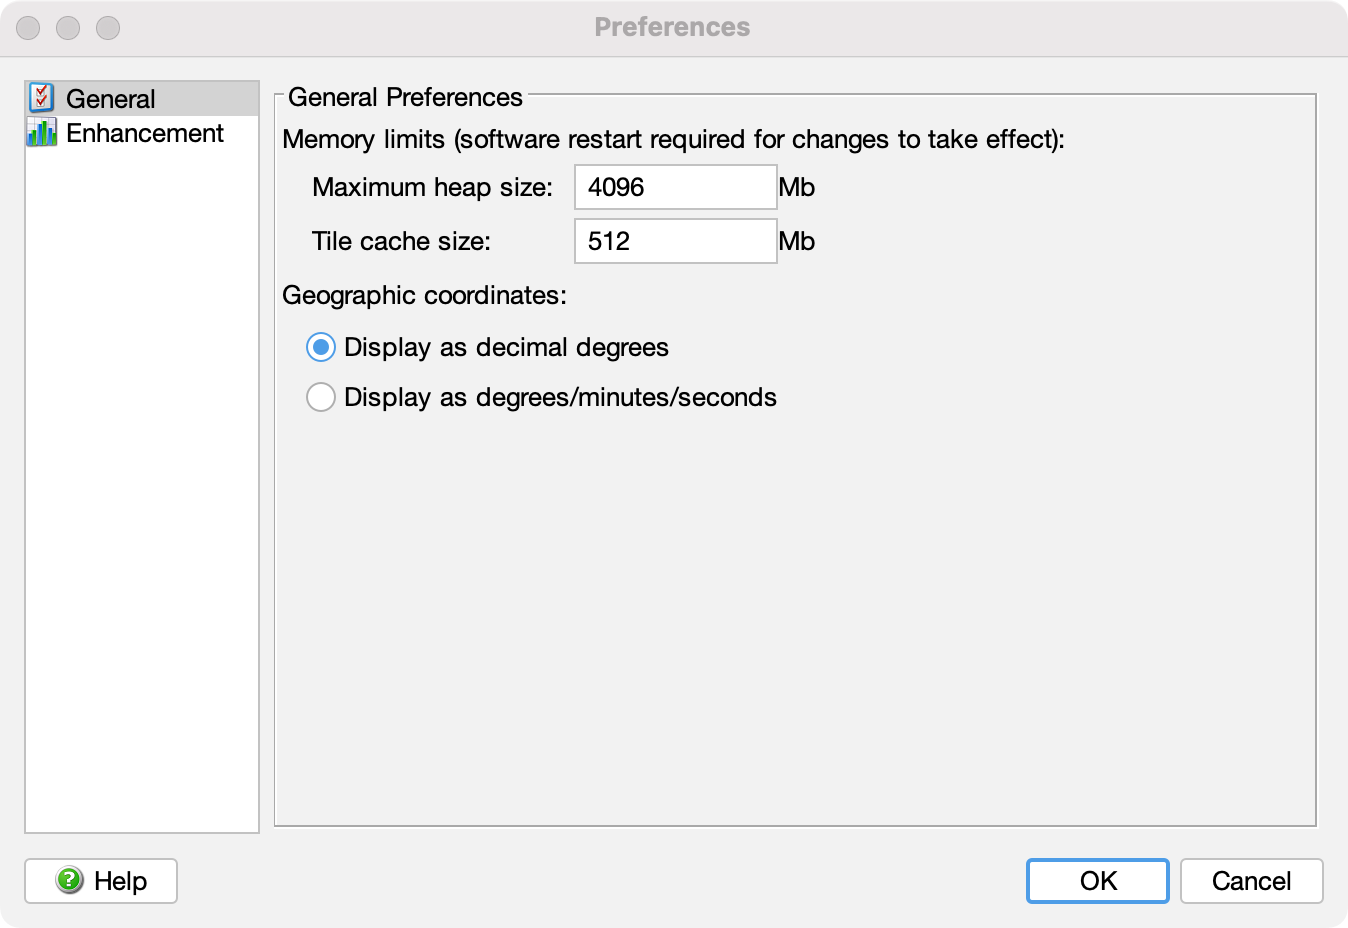
\includegraphics[width=4in]{figures/cdat_general_prefs.png}
    \caption[General section in the Preferences panel]{
       {\gui General} section in the
       \button{preferences}{Preferences} panel
    }
    \label{general_prefs}
  \end{center}
\end{figure}

\subsection{Setting color palette, enhancement, and units}

When a data file is opened and variables are selected, CDAT shows
the initial data view for each variable using a color palette,
enhancement range, and units determined from the user preferences
(see \autoref{loading} on loading data).  Rather than having to
customize all these items each time a data file is opened, you
can set up preferences for each variable name.  CDAT comes with a
set of built-in preferences for a number of common variable
names.  To edit these preferences or add new variables, click
\button{preferences}{Preferences} from the {\gui Tools} menu, then
click \button{column-chart}{Enhancement} for the enhancement
preferences (see \autoref{enhancement_prefs}).  To modify the
settings for a certain variable, click the variable name in the
{\gui Variable} list or type in a new variable name and click
\button{add}{Add} to add it to the list (some default preferences
will be assigned to it that need to be modified).  Once a
variable is selected, you can change various settings:
\begin{description}

\item[Palette] -- Choose one of the palettes from the list.  New
palettes can be added to the list using an XML palette format,
see \autoref{resources}.

\item[Units] -- Keep the same units as in the data file or choose
different units to display the variable data values.  CDAT
normally uses the units that the data file was originally written
with.  For example if a sea surface temperature data variable was
written with Celsius units, then CDAT uses Celsius for all
numerical value readings: the data view track bar, the
\button{column-chart}{Color Enhancement} tab sliders and text
fields, the \button{tape_measure2}{Data Surveys} tab statistics
and plots, and any other location that a numerical value is
displayed.  But if the units are set to ``Display in units of
fahrenheit'', then all numerical readings are shown in Fahrenheit
instead.  If you select different data units, remember to also
modify the {\gui Minimum} and {\gui Maximum} text fields to match
those units.  A number of common units are provided in the
drop-down units box. If your preferred units are not shown, you
can also type in the units. Most common units are supported, and
base units can be combined with spaces, slashes, and
exponentiation. For example, wind or ocean current speed in
kilometers per hour could be written a number of ways: ``km/h'',
``km hr\^{~}-1'', ``kilometers / hour'', or ``kilometers per
hour''.  For other possible unit names, see the
conventions used by the \href{https://www.google.com/search?q=udunits}{Unidata
UDUNITS package} and its \href{https://www.google.com/search?q=udunits.txt}{supported
units} file.

\item[Enhancement function] -- Select the color scale minimum and
maximum values and the type of function: {\gui Linear},
{\gui Step}, or {\gui Log10}. See \autoref{changing_colors} for a
description of the \button{column-chart}{Color Enhancement} tab
where these preferences are used.

\end{description}
After modifying any of the preferences, click {\gui OK} the save
them or {\gui Cancel} to discard all the changes.  Note that
enhancement preferences only take effect the next time a data
file is opened and variables loaded.

\begin{figure}
  \begin{center}
    \myfigure{enhancement_prefs}
    \caption[Enhancement section in the Preferences panel]{
       \button{column-chart}{Enhancement} section in the
       \button{preferences}{Preferences} panel
    }
    \label{enhancement_prefs}
  \end{center}
\end{figure}

\subsection{Resources directory}
\label{resources}

CDAT stores preferences for each user on the system individually.
Depending on the operating system, preferences are stored in a
resources directory under your home directory:
\begin{description}

\item[Windows 2K/XP/2003] -- \verb+\Documents and Settings\[User name]\Application Data\CoastWatch+

\item[Windows Vista/7] -- \verb+\Users\[User name]\AppData\Roaming\CoastWatch+

\item[Mac OS X] -- \verb+~/Library/Application Support/CoastWatch+

\item[Unix] -- \verb+~/.coastwatch+

\end{description}
Preferences are normally modified using the CDAT
\button{preferences}{Preferences} panel but can also be modified
by editing the XML files in the resources directory.  On some
operating systems it may be necessary to show hidden directories
to reveal the resources directory.  {\bf Only attempt to modify
the resources manually if you are familiar with editing XML files
and have made a backup of any files first.}  In the case of some
resource file problem indicated by an error when launching CDAT,
you can delete the resources directory, restart CDAT, and the
resources directory will be recreated and populated with the
default preferences.

The resources directory contains various files and subdirectories
as follows:
\begin{description}

\item[{\tt prefs.xml}] -- Main preferences file with general and
enhancement preferences.

% \item[{\tt opendap\_servers.xml}] -- List of current OPeNDAP
% servers, accessed and edited under the
% \button{harddisk_network}{Network} tab after clicking
% \button{folder_out}{Open}.

\item[{\tt overlays/}] -- Directory for storing overlay groups
from the \button{tables}{Overlay Layers} tab.  Each overlay group
is stored as a separate file with a {\file .jso} extension for
``Java Serialized Object'', a binary format used for
saving/restoring a Java object's state.  Overlay groups can be
copied between computers, even between different operating
systems, although some incompatibilities in overlays may exist
between different CoastWatch Utilities versions.

\item[{\tt palettes/}] -- Directory for storing extra
user-supplied palettes.  Any files with a {\file .xml} extension
will be considered to be palette files and read into CDAT for use
in the \button{palette}{Color Palette} tab and
\button{preferences}{Preferences} panel.  Palette files must have
the format described in \autoref{palette_xml} for color palettes.

\end{description}

Some users have asked ``How can I modify an existing color
palette and use that in CDAT?''  To do this, you can extract it
from the {\file lib/java/cwutils.jar} file in the CoastWatch Utilities
installation directory using the Java jar command in a command
line session, for example:
\begin{verbatim}
  jar xf <path to CW utils>/lib/java/cwutils.jar noaa/coastwatch/render/HSL256.xml
\end{verbatim}
which will extract the HSL256 palette XML file to a {\file noaa}
subdirectory (do this command in some scratch working directory,
not in the {\file lib/} directory).  Then modify the palette file
RGB color triplets, rename the file, change the
\verb+<palette name="...">+ inside the file to match, and copy
the new XML file into the {\file palettes/} directory.  After
restarting CDAT the new palette should appear in the
\button{palette}{Color Palette} tab.

\section{Connections with command line tools}

The CoastWatch Data Analysis Tool can be used on conjunction with
the CoastWatch Utilities command line tools (described in
\autoref{common} and \autoref{manual}) in a number of ways:
\begin{description}

\item[Visualization] -- CDAT can be used to set up a plot's
characteristics for use with the \hyperlink{cwrender}{cwrender}
tool.  You can manually transfer settings from CDAT to the
rendering command line:
\begin{itemize}

  \item Variable being displayed $\rightarrow$ \longoption{enhance}

  \item Enhancement min/max text fields and function
  $\rightarrow$ \longoption{range}, \longoption{function}

  \item Selected color palette $\rightarrow$ \longoption{palette}

  \item Overlay layers $\rightarrow$ \longoption{coast},
  \longoption{grid}, \longoption{political}, \longoption{bath},
  \longoption{group} and others

  \item Units preferences  $\rightarrow$ \longoption{units}

  \item Region shown in data view $\rightarrow$ \longoption{magnify}

  \item Color composite variables $\rightarrow$
  \longoption{composite}

\end{itemize}
Note that custom palettes and overlay groups stored in the user's
resource directory (\autoref{resources}) can also be used by
cwrender.

\item[Statistics] -- To perform a similar box data survey from a
script as was performed using the \button{tape_measure2}{Data
Surveys} tab \button{bullet_ball_glass_blue_box}{Box} mode
(\autoref{surveys}), you can either (i) hover the mouse cursor
over the center of the box and note the latitude and longitude
value to use in the \longoption{region} option to the
\hyperlink{cwstats}{cwstats} tool, or (ii) note the box corner
row and column values from the survey results for the
\longoption{limit} option.

\item[Sampling] -- To perform a similar point data survey from
the command line as was performed using the
\button{tape_measure2}{Data Surveys} tab \button{pin_blue}{Point}
mode, you can note the latitude and longitude values in the point
survey results and use them for the \longoption{sample} option in
the \hyperlink{cwsample}{cwsample} tool.  Multiple variables in a
data file can be sampled at once using cwsample, rather than CDAT
which only surveys the displayed variable.

\item[Navigation] -- After using the {\gui Navigation Analysis} panel
(\autoref{nav_analysis_section}) to determine the best navigation
correction for the data file, you can apply/reset the navigation
correction using the \hyperlink{cwnavigate}{cwnavigate} tool.
If you save a number of navigation points that would likely be
good for future navigation efforts, their latitude/longitude
coordinates could be used as input to the
\hyperlink{cwautonav}{cwautonav} tool.

\item[Export] -- The CDAT \button{export2}{Export} button
(\autoref{exporting}) has almost the same functionality as the
\hyperlink{cwrender}{cwrender} and \hyperlink{cwexport}{cwexport}
tools combined.  The {\gui Format} box in the CDAT {\gui Export}
window has the same color image formats as the
\longoption{format} option in cwrender, and the same numerical
data formats as \longoption{format} in cwexport.  CDAT export
options map to the command line as follows:
\begin{itemize}

\item Color image options $\rightarrow$ \longoption{nolegends},
\longoption{tiffcomp}, \longoption{worldfile},
\longoption{noantialias}, \longoption{imagecolors} in cwrender

\item Numerical data options $\rightarrow$ \longoption{header},
\longoption{match}, \longoption{missing}, \longoption{scale},
\longoption{range}, \longoption{byteorder}, \longoption{size},
\longoption{nocoords}, \longoption{reverse} in cwexport

\end{itemize}

\item[File information] -- The file information shown by clicking
{\gui Tools | File Information} in CDAT is the same as that
reported by the \hyperlink{cwinfo}{cwinfo} tool.  The file information window
in CDAT also has a raw metadata search and display that shows
the same metadata values as the \hyperlink{hdatt}{hdatt} tool or the NetCDF 
software ncdump program.

\item[Data formats] -- The same data formats read by CDAT can be read by 
most of the command line tools.  See \autoref{compatible} for more details on
data format compatibility between tools.

\end{description}
